\chapter{De redes soma-produto para redes bayesianas}
\label{cap:desenvolvimento}

Enquanto as redes bayesianas são visualizações gráficas de dependências diretas e redes de Markov são visualizações gráficas de correlações, as redes soma-produto são visualizações gráficas de computações \cite{Poupart2017}.

Desde a introdução de SPNs no trabalho de Poon e Domingos \cite{Poon2012}, esteve claro que as SPNs e BNs são igualmente expressivas no sentido que elas podem representar qualquer distribuição conjunta sobre variáveis discretas. Entretanto, apenas em 2015 foi provado, por Zhao \emph{et al.} \cite{Zhao2015}, que toda rede soma-produto pode ser convertida numa rede bayesiana em complexidade linear de tempo e espaço no tamanho da SPN.

Tal artigo apresenta um algoritmo para realizar essa conversão, que foi estudado e implementado neste trabalho.

\section{Algoritmo de Zhao \emph{et al.}}

Dada uma SPN normal $\mathcal{S}$ sobre variáveis booleanas $X_{1:N}$, o algoritmo de Zhao \emph{et al.} \cite{Zhao2015} retorna uma rede bayesiana $\mathcal{B}$ que representa a mesma distribuição com $|\mathcal{B}| = O(N|\mathcal{S}|)$. Pode-se explicar o algoritmo mais facilmente separando-o em duas etapas:

\begin{enumerate}
  \item Construção da estrutura da rede bayesiana;
  \item Computação das distribuições de probabilidade condicional (\emph{CPD}, do inglês \emph{conditional probability distribution}).
\end{enumerate}

\subsection{Construção da estrutura}

A rede bayesiana resultante terá dois tipos de variáveis: observáveis e ocultas. As variáveis observáveis correspondem a variáveis de $\mathcal{S}$, enquanto as variáveis ocultas correspondem a nós soma de $\mathcal{S}$.

Para construir a estrutura da BN, portanto, deve-se criar nós para cada variável de $\mathcal{S}$ e para cada nó soma de $\mathcal{S}$. Os nós da BN associados aos nós soma da SPN tem arestas direcionadas para todas as variáveis do seu escopo.

Logo, a rede bayesiana terá uma estrutura bipartida. As variáveis ocultas terão apenas grau de saída, enquanto as variáveis observáveis terão apenas grau de entrada. A figura \ref{fig:algorithm} (a) mostra como fica a estrutura da rede bayesiana que corresponde a conversão da SPN normal vista na figura \ref{fig:spn} (c).

\begin{figure}
  \begin{minipage}{0.3333\textwidth}
    \centering
    \scalebox{1.1}{
      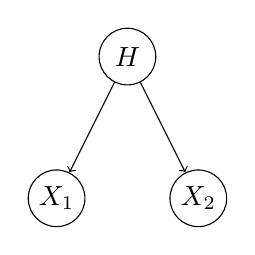
\begin{tikzpicture}
          [scale=.6,auto=left,every node/.style={draw, circle, inner sep = 0pt, minimum width = 0.72cm}]
        \node (n1) at (5,10) {$H$};
        \node (n56) at (3.5,7) {$X_1$};
        \node (n78) at (6.5,7) {$X_2$};

        \foreach \from/\to in {n1/n56, n1/n78}
          \draw (\from) edge[->] (\to);
      \end{tikzpicture}
    }

    (a)
  \end{minipage}\begin{minipage}{0.3333\textwidth}
    \centering
    \scalebox{0.8}{
      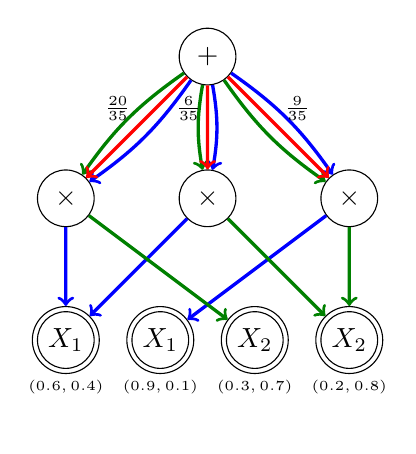
\begin{tikzpicture}
          [scale=.6,auto=left,every node/.style={draw, circle, inner sep = 0pt, minimum width = 0.72cm}]
        \node (n1) at (5,10) {$+$};
        \node (n2) at (2,7) {$\times$};
        \node (n3) at (5,7) {$\times$};
        \node (n4) at (8,7) {$\times$};
        \node (n5) at (2,4) {$X_1$};
        \node (n6) at (4,4) {$X_1$};
        \node (n7) at (6,4) {$X_2$};
        \node (n8) at (8,4) {$X_2$};

        \node[minimum width = 0.85cm] (n5) at (2,4) {};
        \node[minimum width = 0.85cm] (n6) at (4,4) {};
        \node[minimum width = 0.85cm] (n7) at (6,4) {};
        \node[minimum width = 0.85cm] (n8) at (8,4) {};

        \node[draw=none] (n9) at (2,3) {\tiny $(0.6, 0.4)$};
        \node[draw=none] (n10) at (4,3) {\tiny $(0.9, 0.1)$};
        \node[draw=none] (n11) at (6,3) {\tiny $(0.3, 0.7)$};
        \node[draw=none] (n12) at (8,3) {\tiny $(0.2, 0.8)$};

        \foreach \from/\to in {n1/n2, n1/n3, n1/n4}
          \draw[very thick,draw=Blue] (\from) edge[->, bend left=10] (\to);

        \foreach \from/\to in {n1/n2, n1/n3, n1/n4}
          \draw[very thick,draw=Green] (\from) edge[->, bend right=10] (\to);

        \foreach \from/\to/\weight/\pos in {n1/n2/$\frac{20}{35}$/above left, n1/n3/$\frac{6}{35}$/above left, n1/n4/$\frac{9}{35}$/above right}
          \draw[very thick,draw=Red] (\from) edge[->] node[\pos, draw=none, circle=none, minimum width=0.5cm, minimum height=0.2cm, inner sep=2pt]{\scriptsize \weight} (\to);

        \foreach \from/\to in {n2/n5, n3/n5, n4/n6}
          \draw[very thick,draw=Blue] (\from) edge[->] (\to);

        \foreach \from/\to in {n2/n7, n3/n8, n4/n8}
          \draw[very thick,draw=Green] (\from) edge[->] (\to);
      \end{tikzpicture}
    }

    (b)
  \end{minipage}\begin{minipage}{0.3333\textwidth}
    \centering
    \scalebox{0.45}{
      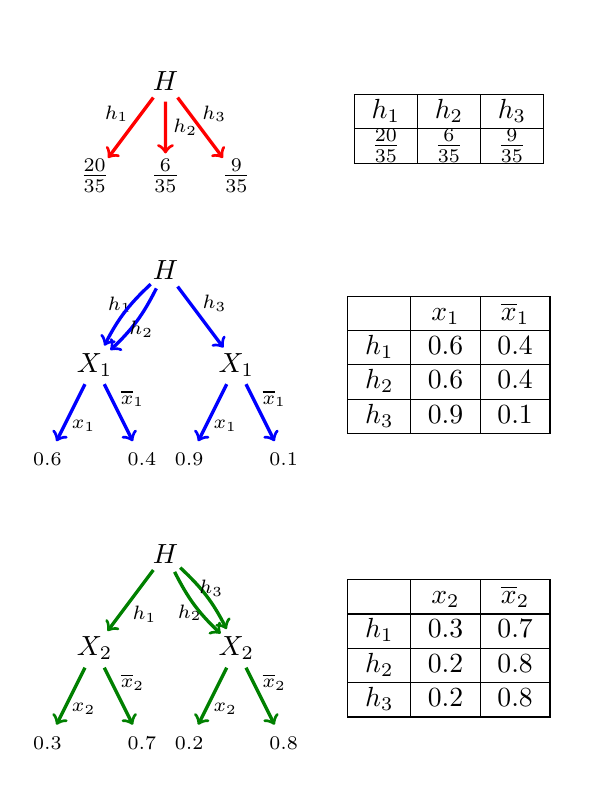
\begin{tikzpicture}
          [scale=.6,auto=left,every node/.style={draw, circle, inner sep = 0pt, minimum width = 0.72cm}]
        \node[draw=none, minimum width = 0.5cm] (rH) at (3,20) {$H$};
        \node[draw=none, minimum width = 0.5cm] (rh1) at (1.5,18) {$\frac{20}{35}$};
        \node[draw=none, minimum width = 0.5cm] (rh2) at (3,18) {$\frac{6}{35}$};
        \node[draw=none, minimum width = 0.5cm] (rh3) at (4.5,18) {$\frac{9}{35}$};

        \draw[very thick,draw=Red] (rH) edge[->] node[above left, draw=none, circle=none, minimum width=0.3cm, minimum height=0.2cm, inner sep=1pt]{\scriptsize $h_1$} (rh1);
        \draw[very thick,draw=Red] (rH) edge[->] node[draw=none, circle=none, minimum width=0.3cm, minimum height=0.2cm, inner sep=1pt]{\scriptsize $h_2$} (rh2);
        \draw[very thick,draw=Red] (rH) edge[->] node[draw=none, circle=none, minimum width=0.3cm, minimum height=0.2cm, inner sep=1pt]{\scriptsize $h_3$} (rh3);

        \node[draw=none, minimum width = 0.5cm] (bH) at (3,16) {$H$};
        \node[draw=none, minimum width = 0.5cm] (bh12) at (1.5,14) {$X_1$};
        \node[draw=none, minimum width = 0.5cm] (bh3) at (4.5,14) {$X_1$};
        \node[draw=none, minimum width = 0.5cm] (bx1a) at (0.5,12) {\scriptsize $0.6$};
        \node[draw=none, minimum width = 0.5cm] (bnx1a) at (2.5,12) {\scriptsize $0.4$};
        \node[draw=none, minimum width = 0.5cm] (bx1b) at (3.5,12) {\scriptsize $0.9$};
        \node[draw=none, minimum width = 0.5cm] (bnx1b) at (5.5,12) {\scriptsize $0.1$};

        \draw[very thick,draw=Blue] (bH) edge[->, bend left=10] node[above left, draw=none, circle=none, minimum width=0.3cm, minimum height=0.2cm, inner sep=2pt]{\scriptsize $h_1$} (bh12);
        \draw[very thick,draw=Blue] (bH) edge[->, bend right=10] node[below right, draw=none, circle=none, minimum width=0.3cm, minimum height=0.2cm, inner sep=2pt]{\scriptsize $h_2$} (bh12);
        \draw[very thick,draw=Blue] (bH) edge[->] node[draw=none, circle=none, minimum width=0.3cm, minimum height=0.2cm, inner sep=1pt]{\scriptsize $h_3$} (bh3);

        \draw[very thick,draw=Blue] (bh12) edge[->] node[draw=none, circle=none, minimum width=0.3cm, minimum height=0.2cm, inner sep=1pt]{\scriptsize $x_1$} (bx1a);
        \draw[very thick,draw=Blue] (bh12) edge[->] node[draw=none, circle=none, minimum width=0.3cm, minimum height=0.2cm, inner sep=1pt]{\scriptsize $\overline x_1$} (bnx1a);
        \draw[very thick,draw=Blue] (bh3) edge[->] node[draw=none, circle=none, minimum width=0.3cm, minimum height=0.2cm, inner sep=1pt]{\scriptsize $x_1$} (bx1b);
        \draw[very thick,draw=Blue] (bh3) edge[->] node[draw=none, circle=none, minimum width=0.3cm, minimum height=0.2cm, inner sep=1pt]{\scriptsize $\overline x_1$} (bnx1b);

        \node[draw=none, minimum width = 0.5cm] (gH) at (3,10) {$H$};
        \node[draw=none, minimum width = 0.5cm] (gh1) at (1.5,8) {$X_2$};
        \node[draw=none, minimum width = 0.5cm] (gh23) at (4.5,8) {$X_2$};
        \node[draw=none, minimum width = 0.5cm] (gx2a) at (0.5,6) {\scriptsize $0.3$};
        \node[draw=none, minimum width = 0.5cm] (gnx2a) at (2.5,6) {\scriptsize $0.7$};
        \node[draw=none, minimum width = 0.5cm] (gx2b) at (3.5,6) {\scriptsize $0.2$};
        \node[draw=none, minimum width = 0.5cm] (gnx2b) at (5.5,6) {\scriptsize $0.8$};

        \draw[very thick,draw=Green] (gH) edge[->] node[draw=none, circle=none, minimum width=0.3cm, minimum height=0.2cm, inner sep=1pt]{\scriptsize $h_1$} (gh1);
        \draw[very thick,draw=Green] (gH) edge[->, bend left=10] node[below left, draw=none, circle=none, minimum width=0.3cm, minimum height=0.2cm, inner sep=2pt]{\scriptsize $h_2$} (gh23);
        \draw[very thick,draw=Green] (gH) edge[->, bend right=10] node[above right, draw=none, circle=none, minimum width=0.3cm, minimum height=0.2cm, inner sep=2pt]{\scriptsize $h_3$} (gh23);

        \draw[very thick,draw=Green] (gh1) edge[->] node[draw=none, circle=none, minimum width=0.3cm, minimum height=0.2cm, inner sep=1pt]{\scriptsize $x_2$} (gx2a);
        \draw[very thick,draw=Green] (gh1) edge[->] node[draw=none, circle=none, minimum width=0.3cm, minimum height=0.2cm, inner sep=1pt]{\scriptsize $\overline x_2$} (gnx2a);
        \draw[very thick,draw=Green] (gh23) edge[->] node[draw=none, circle=none, minimum width=0.3cm, minimum height=0.2cm, inner sep=1pt]{\scriptsize $x_2$} (gx2b);
        \draw[very thick,draw=Green] (gh23) edge[->] node[draw=none, circle=none, minimum width=0.3cm, minimum height=0.2cm, inner sep=1pt]{\scriptsize $\overline x_2$} (gnx2b);

        \node[draw=none,inner sep = 0pt] at (9,19)
        {
          \begin{tabular}{|c|c|c|} \hline
            $h_1$ & $h_2$ & $h_3$ \\ \hline
            $\frac{20}{35}$ & $\frac{6}{35}$ & $\frac{9}{35}$ \\ \hline
          \end{tabular}
        };

        \node[draw=none,inner sep = 0pt] at (9,14)
        {
          \begin{tabular}{|c|c|c|} \hline
                  & $x_1$ & $\overline x_1$ \\ \hline
            $h_1$ & $0.6$ & $0.4$ \\ \hline
            $h_2$ & $0.6$ & $0.4$ \\ \hline
            $h_3$ & $0.9$ & $0.1$ \\ \hline
          \end{tabular}
        };

        \node[draw=none,inner sep = 0pt] at (9,8)
        {
          \begin{tabular}{|c|c|c|} \hline
                  & $x_2$ & $\overline x_2$ \\ \hline
            $h_1$ & $0.3$ & $0.7$ \\ \hline
            $h_2$ & $0.2$ & $0.8$ \\ \hline
            $h_3$ & $0.2$ & $0.8$ \\ \hline
          \end{tabular}
        };
      \end{tikzpicture}
    }

    (c)
  \end{minipage}

  \caption{
    \textbf{(a)} Estrutura da rede bayesiana correspondente à SPN normal vista na figura \ref{fig:spn} (c).
    \textbf{(b)} Sub-SPNs induzidas usadas para construir os diagramas de decisão algébrica.
    \textbf{(c)} Distribuições de probabilidade condicional calculados para a rede bayesiana convertida (diagramas de decisão algébrica e tabelas equivalentes).
  }
  \label{fig:algorithm}
\end{figure}

\subsection{Distribuições de probabilidade condicional}

Apresentaremos primeiro as distribuições de probabilidade condicional das variáveis ocultas e depois das variáveis observáveis.

\vspace{1em}

Se $H_v$ é a variável oculta correspondente ao nó soma $v$ de $\mathcal{S}$ e $l$ é o grau de saída de $v$, como $mathcal{S}$ é normal, temos $\sum_{i=1}^l w_i = 1$ e $w_i \geq 0 \quad \forall i$. Isso sugere tomar $P(H_v = i) = w_i$.

\vspace{1em}

Agora fixemos uma variável observável $X$. Sejam $H_{v_1}, \cdots, H_{v_k}$ as variáveis ocultas que apontam para ela na rede bayesiana. Precisamos definir $P(X | H_{v_1} = v_1^*, \cdots, H_{v_m} = v_m^*)$ para cada combinação de $v_1^*, \cdots, v_m^*$ (valores que as variáveis ocultas $H_{v_1}, \cdots, H_{v_m}$ podem assumir).

A ideia para fazer isso vem da Proposição 1 do artigo \cite{Zhao2015}:

\begin{proposition}
  Seja $p$ um nó produto em $\mathcal{S}$ com $l$ filhos. Sejam $p_1, \cdots, p_l$ os filhos de $p$. Sejam $v_1, \cdots, v_k$ os nós soma no caminho da raiz de $\mathcal{S}$ até $p$. Então

  \begin{multline}
    \displaystyle P(X_{|\textrm{escopo}(p)} | H_{v_1} = v_1^*, \cdots, H_{v_k} = v_k^*) =\\
    \prod_{i = 1}^l P(X_{|\textrm{escopo}(p_i)} | H_{v_1} = v_1^*, \cdots, H_{v_k} = v_k^*)
  \end{multline}

  onde $H_v = v^*$ significa que o nó soma $v$ seleciona seu $v^*$-ésimo filho e $X_{|A}$ denota a restrição de $X$ pelo conjunto $A$.
\end{proposition}

Como a SPN é decomponível, cada nó produto tem filhos com escopos disjuntos. Para cada variável observável $X$, construímos um ADD extraindo de $\mathcal{S}$ a sub-SPN induzida por $X$ e contraindo todos seus nós produto. Percorremos o ADD para encontrar $P(X | H_{v_1} = v_1^*, \cdots, H_{v_m} = v_m^*)$.

A figura \ref{fig:algorithm} (b) mostra as as sub-SPNs induzidas usadas para criar os diagramas de decisão algébrica da rede bayesiana na figura \ref{fig:algorithm} (a). A figura \ref{fig:algorithm} (c) mostra os ADDs resultantes e as tabelas de CPDs equivalentes a esses ADDs.

Zhao \emph{et al.} \cite{Zhao2015} apresenta uma prova para o algoritmo por indução na altura de $\mathcal{S}$.

\section{Implementação}

A implementação desse algoritmo foi realizada na linguagem Go\footnote{\emph{The Go Programming Language:} \url{https://golang.org/}}. \emph{Go} é uma linguagem de código aberto criada em 2007 e apoiada pelo \emph{Google}. Ela é compilada e usa tipagem estática como o C, mas possui recursos avançados como \emph{garbage collection} e bom suporte a programação concorrente. Escolhemos \emph{Go} porque ela oferece um bom balanço entre a agilidade de escrita de código e a eficiência computacional; tem sistemas de pacotes ({\tt go get}), testes ({\tt go test}) e documentação (\emph{GoDoc}\footnote{\emph{GoDoc:} \url{https://godoc.org/}}) padronizados facilitando que os códigos sejam testados e reutilizados; e ajuda a gerar código limpo e padronizado: indentação, espaçamento e outros detalhes de estilo são automatizados pela ferramenta {\tt gofmt}.

Foram desenvolvidos quatro pacotes:

\begin{itemize}
  \item {\tt add}: estrutura de dados que representa diagramas de decisão algébrica
  \item {\tt bn}: estrutura de dados que representa redes bayesianas com CPDs representados por ADDs
  \item {\tt spn}: estrutura de dados que representa redes soma-produto
  \item {\tt zhao:} implementação do algoritmo
\end{itemize}

Eles foram disponibilizados publicamente em \url{https://github.com/tmadeira/spnbn}. Um exemplo de uso do algoritmo pode ser visto em {\tt examples/a/a.go}. Tal código cria a rede soma-produto {\tt S} vista na figura \ref{fig:spn} (c) e usa o algoritmo chamando {\tt zhao.BuildBN(S)}:

\lstinputlisting[firstline=22, lastline=43]{../implementacao/spnbn/examples/a/a.go}

\section{Exemplos}

A figura \ref{fig:ex1} (a) mostra uma SPN $\mathcal{T}$ construída a partir da duplicação da SPN apresentada na figura \ref{fig:spn} (c) e da adição se um nó produto que aponta para a rede original e para sua cópia.

Como se pode perceber, a rede bayesiana resultante da conversão usando o algoritmo implementado neste trabalho, apresentada na figura \ref{fig:ex1} (b), é um grafo desconexo, separado em dois subgrafos bipartidos exatamente iguais ao visto na figura \ref{fig:algorithm}.

Já que não são adicionados nós soma, não há nenhuma nova variável oculta na rede bayesiana resultante. Como não há nenhum nó soma que tenha como escopo uma variável entre $X_1, X_2$ e outra entre $X_3, X_4$ o grafo acaba ficando desconexo. Como se pode esperar, portanto, a adição de um nó produto na raiz não tem muita utilidade no sentido de mudar o entendimento da semântica probabilística da estrutura.

Esse exemplo pode ser visto no arquivo {\tt examples/b/b.go} disponibilizado junto com a implementação do algoritmo.

\begin{figure}
  \begin{minipage}{0.5\textwidth}
    \centering
    \scalebox{0.6}{
      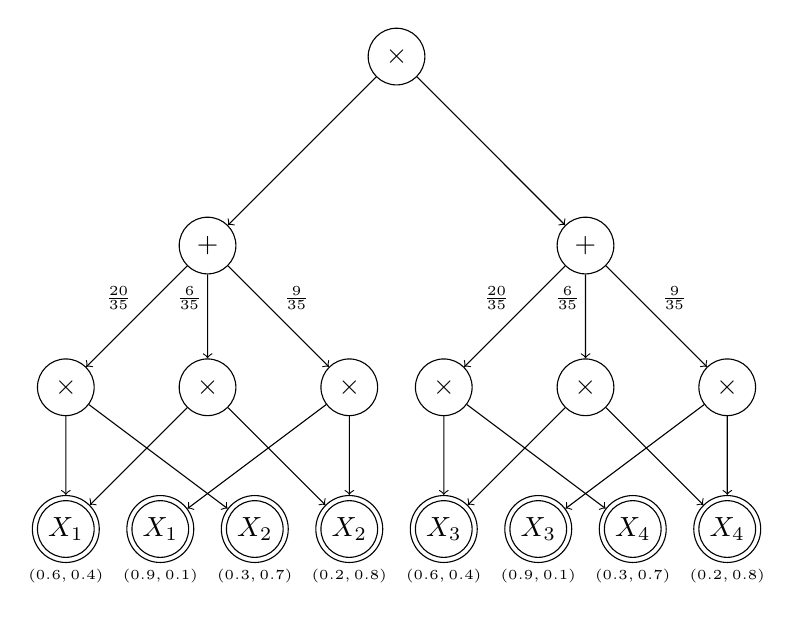
\begin{tikzpicture}
          [scale=.6,auto=left,every node/.style={draw, circle, inner sep = 0pt, minimum width = 0.72cm}]
        \node (n1) at (5,10) {$+$};
        \node (n2) at (2,7) {$\times$};
        \node (n3) at (5,7) {$\times$};
        \node (n4) at (8,7) {$\times$};
        \node (n5) at (2,4) {$X_1$};
        \node (n6) at (4,4) {$X_1$};
        \node (n7) at (6,4) {$X_2$};
        \node (n8) at (8,4) {$X_2$};

        \node[minimum width = 0.85cm] (n5) at (2,4) {};
        \node[minimum width = 0.85cm] (n6) at (4,4) {};
        \node[minimum width = 0.85cm] (n7) at (6,4) {};
        \node[minimum width = 0.85cm] (n8) at (8,4) {};

        \node[draw=none] (n9) at (2,3) {\tiny $(0.6, 0.4)$};
        \node[draw=none] (n10) at (4,3) {\tiny $(0.9, 0.1)$};
        \node[draw=none] (n11) at (6,3) {\tiny $(0.3, 0.7)$};
        \node[draw=none] (n12) at (8,3) {\tiny $(0.2, 0.8)$};

        \foreach \from/\to/\weight/\pos in {n1/n2/$\frac{20}{35}$/above left, n1/n3/$\frac{6}{35}$/above left, n1/n4/$\frac{9}{35}$/above right}
          \draw (\from) edge[->] node[\pos, draw=none, circle=none, minimum width=0.5cm, minimum height=0.2cm, inner sep=2pt]{\scriptsize \weight} (\to);

        \foreach \from/\to in {n2/n5, n2/n7, n3/n5, n3/n8, n4/n6, n4/n8}
          \draw (\from) edge[->] (\to);

        \node (m1) at (13,10) {$+$};
        \node (m2) at (10,7) {$\times$};
        \node (m3) at (13,7) {$\times$};
        \node (m4) at (16,7) {$\times$};
        \node (m5) at (10,4) {$X_3$};
        \node (m6) at (12,4) {$X_3$};
        \node (m7) at (14,4) {$X_4$};
        \node (m8) at (16,4) {$X_4$};

        \node[minimum width = 0.85cm] (m5) at (10,4) {};
        \node[minimum width = 0.85cm] (m6) at (12,4) {};
        \node[minimum width = 0.85cm] (m7) at (14,4) {};
        \node[minimum width = 0.85cm] (m8) at (16,4) {};

        \node[draw=none] (m9) at (10,3) {\tiny $(0.6, 0.4)$};
        \node[draw=none] (m10) at (12,3) {\tiny $(0.9, 0.1)$};
        \node[draw=none] (m11) at (14,3) {\tiny $(0.3, 0.7)$};
        \node[draw=none] (m12) at (16,3) {\tiny $(0.2, 0.8)$};

        \foreach \from/\to/\weight/\pos in {m1/m2/$\frac{20}{35}$/above left, m1/m3/$\frac{6}{35}$/above left, m1/m4/$\frac{9}{35}$/above right}
          \draw (\from) edge[->] node[\pos, draw=none, circle=none, minimum width=0.5cm, minimum height=0.2cm, inner sep=2pt]{\scriptsize \weight} (\to);

        \foreach \from/\to in {m2/m5, m2/m7, m3/m5, m3/m8, m4/m6, m4/m8}
          \draw (\from) edge[->] (\to);

        \node (nm) at (9,14) {$\times$};

        \draw (nm) edge[->] (n1);
        \draw (nm) edge[->] (m1);
      \end{tikzpicture}
    }

    (a)
  \end{minipage}\begin{minipage}{0.5\textwidth}
    \centering
    \scalebox{0.6}{
      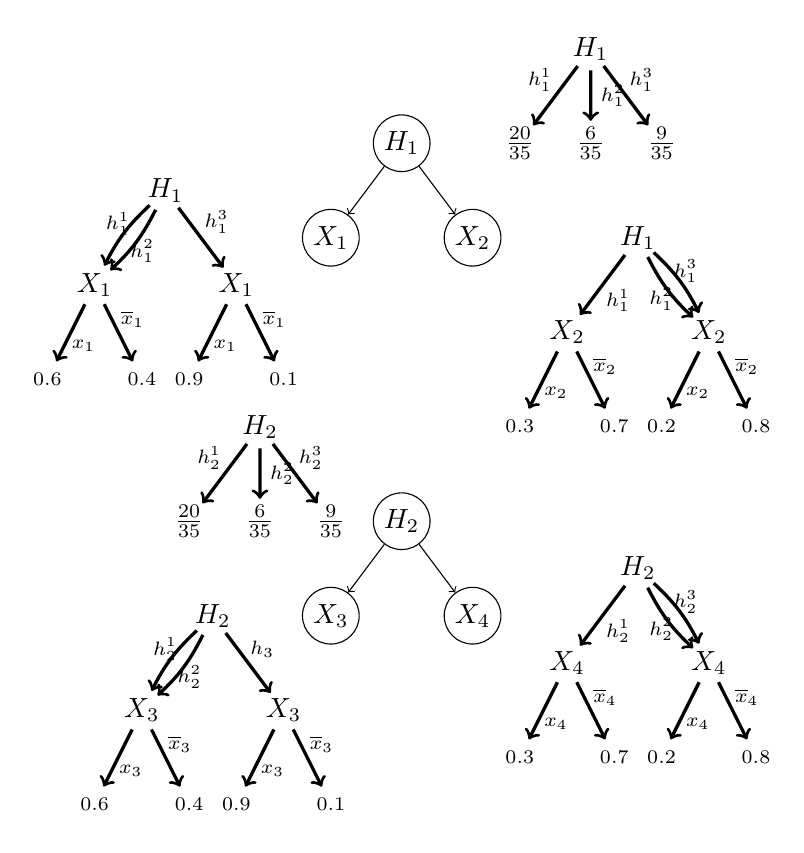
\begin{tikzpicture}
          [scale=.6,auto=left,every node/.style={draw, circle, inner sep = 0pt, minimum width = 0.72cm}]
        \node (n1) at (5,19) {$H_1$};
        \node (n56) at (3.5,17) {$X_1$};
        \node (n78) at (6.5,17) {$X_2$};

        \foreach \from/\to in {n1/n56, n1/n78}
          \draw (\from) edge[->] (\to);

        \node[draw=none, minimum width = 0.5cm] (rH) at (9,21) {$H_1$};
        \node[draw=none, minimum width = 0.5cm] (rh1) at (7.5,19) {$\frac{20}{35}$};
        \node[draw=none, minimum width = 0.5cm] (rh2) at (9,19) {$\frac{6}{35}$};
        \node[draw=none, minimum width = 0.5cm] (rh3) at (10.5,19) {$\frac{9}{35}$};

        \draw[very thick] (rH) edge[->] node[above left, draw=none, circle=none, minimum width=0.3cm, minimum height=0.2cm, inner sep=1pt]{\scriptsize $h_1^1$} (rh1);
        \draw[very thick] (rH) edge[->] node[draw=none, circle=none, minimum width=0.3cm, minimum height=0.2cm, inner sep=1pt]{\scriptsize $h_1^2$} (rh2);
        \draw[very thick] (rH) edge[->] node[draw=none, circle=none, minimum width=0.3cm, minimum height=0.2cm, inner sep=1pt]{\scriptsize $h_1^3$} (rh3);

        \node[draw=none, minimum width = 0.5cm] (bH) at (0,18) {$H_1$};
        \node[draw=none, minimum width = 0.5cm] (bh12) at (-1.5,16) {$X_1$};
        \node[draw=none, minimum width = 0.5cm] (bh3) at (1.5,16) {$X_1$};
        \node[draw=none, minimum width = 0.5cm] (bx1a) at (-2.5,14) {\scriptsize $0.6$};
        \node[draw=none, minimum width = 0.5cm] (bnx1a) at (-0.5,14) {\scriptsize $0.4$};
        \node[draw=none, minimum width = 0.5cm] (bx1b) at (0.5,14) {\scriptsize $0.9$};
        \node[draw=none, minimum width = 0.5cm] (bnx1b) at (2.5,14) {\scriptsize $0.1$};

        \draw[very thick] (bH) edge[->, bend left=10] node[above left, draw=none, circle=none, minimum width=0.3cm, minimum height=0.2cm, inner sep=2pt]{\scriptsize $h_1^1$} (bh12);
        \draw[very thick] (bH) edge[->, bend right=10] node[below right, draw=none, circle=none, minimum width=0.3cm, minimum height=0.2cm, inner sep=2pt]{\scriptsize $h_1^2$} (bh12);
        \draw[very thick] (bH) edge[->] node[draw=none, circle=none, minimum width=0.3cm, minimum height=0.2cm, inner sep=1pt]{\scriptsize $h_1^3$} (bh3);

        \draw[very thick] (bh12) edge[->] node[draw=none, circle=none, minimum width=0.3cm, minimum height=0.2cm, inner sep=1pt]{\scriptsize $x_1$} (bx1a);
        \draw[very thick] (bh12) edge[->] node[draw=none, circle=none, minimum width=0.3cm, minimum height=0.2cm, inner sep=1pt]{\scriptsize $\overline x_1$} (bnx1a);
        \draw[very thick] (bh3) edge[->] node[draw=none, circle=none, minimum width=0.3cm, minimum height=0.2cm, inner sep=1pt]{\scriptsize $x_1$} (bx1b);
        \draw[very thick] (bh3) edge[->] node[draw=none, circle=none, minimum width=0.3cm, minimum height=0.2cm, inner sep=1pt]{\scriptsize $\overline x_1$} (bnx1b);

        \node[draw=none, minimum width = 0.5cm] (gH) at (10,17) {$H_1$};
        \node[draw=none, minimum width = 0.5cm] (gh1) at (8.5,15) {$X_2$};
        \node[draw=none, minimum width = 0.5cm] (gh23) at (11.5,15) {$X_2$};
        \node[draw=none, minimum width = 0.5cm] (gx2a) at (7.5,13) {\scriptsize $0.3$};
        \node[draw=none, minimum width = 0.5cm] (gnx2a) at (9.5,13) {\scriptsize $0.7$};
        \node[draw=none, minimum width = 0.5cm] (gx2b) at (10.5,13) {\scriptsize $0.2$};
        \node[draw=none, minimum width = 0.5cm] (gnx2b) at (12.5,13) {\scriptsize $0.8$};

        \draw[very thick] (gH) edge[->] node[draw=none, circle=none, minimum width=0.3cm, minimum height=0.2cm, inner sep=1pt]{\scriptsize $h_1^1$} (gh1);
        \draw[very thick] (gH) edge[->, bend left=10] node[below left, draw=none, circle=none, minimum width=0.3cm, minimum height=0.2cm, inner sep=2pt]{\scriptsize $h_1^2$} (gh23);
        \draw[very thick] (gH) edge[->, bend right=10] node[above right, draw=none, circle=none, minimum width=0.3cm, minimum height=0.2cm, inner sep=2pt]{\scriptsize $h_1^3$} (gh23);

        \draw[very thick] (gh1) edge[->] node[draw=none, circle=none, minimum width=0.3cm, minimum height=0.2cm, inner sep=1pt]{\scriptsize $x_2$} (gx2a);
        \draw[very thick] (gh1) edge[->] node[draw=none, circle=none, minimum width=0.3cm, minimum height=0.2cm, inner sep=1pt]{\scriptsize $\overline x_2$} (gnx2a);
        \draw[very thick] (gh23) edge[->] node[draw=none, circle=none, minimum width=0.3cm, minimum height=0.2cm, inner sep=1pt]{\scriptsize $x_2$} (gx2b);
        \draw[very thick] (gh23) edge[->] node[draw=none, circle=none, minimum width=0.3cm, minimum height=0.2cm, inner sep=1pt]{\scriptsize $\overline x_2$} (gnx2b);

        \node (m1) at (5,11) {$H_2$};
        \node (m56) at (3.5,9) {$X_3$};
        \node (m78) at (6.5,9) {$X_4$};

        \foreach \from/\to in {m1/m56, m1/m78}
          \draw (\from) edge[->] (\to);

        \node[draw=none, minimum width = 0.5cm] (mrH) at (2,13) {$H_2$};
        \node[draw=none, minimum width = 0.5cm] (mrh1) at (0.5,11) {$\frac{20}{35}$};
        \node[draw=none, minimum width = 0.5cm] (mrh2) at (2,11) {$\frac{6}{35}$};
        \node[draw=none, minimum width = 0.5cm] (mrh3) at (3.5,11) {$\frac{9}{35}$};

        \draw[very thick] (mrH) edge[->] node[above left, draw=none, circle=none, minimum width=0.3cm, minimum height=0.2cm, inner sep=1pt]{\scriptsize $h_2^1$} (mrh1);
        \draw[very thick] (mrH) edge[->] node[draw=none, circle=none, minimum width=0.3cm, minimum height=0.2cm, inner sep=1pt]{\scriptsize $h_2^2$} (mrh2);
        \draw[very thick] (mrH) edge[->] node[draw=none, circle=none, minimum width=0.3cm, minimum height=0.2cm, inner sep=1pt]{\scriptsize $h_2^3$} (mrh3);

        \node[draw=none, minimum width = 0.5cm] (mbH) at (1,9) {$H_2$};
        \node[draw=none, minimum width = 0.5cm] (mbh12) at (-0.5,7) {$X_3$};
        \node[draw=none, minimum width = 0.5cm] (mbh3) at (2.5,7) {$X_3$};
        \node[draw=none, minimum width = 0.5cm] (mbx1a) at (-1.5,5) {\scriptsize $0.6$};
        \node[draw=none, minimum width = 0.5cm] (mbnx1a) at (0.5,5) {\scriptsize $0.4$};
        \node[draw=none, minimum width = 0.5cm] (mbx1b) at (1.5,5) {\scriptsize $0.9$};
        \node[draw=none, minimum width = 0.5cm] (mbnx1b) at (3.5,5) {\scriptsize $0.1$};

        \draw[very thick] (mbH) edge[->, bend left=10] node[above left, draw=none, circle=none, minimum width=0.3cm, minimum height=0.2cm, inner sep=2pt]{\scriptsize $h_2^1$} (mbh12);
        \draw[very thick] (mbH) edge[->, bend right=10] node[below right, draw=none, circle=none, minimum width=0.3cm, minimum height=0.2cm, inner sep=2pt]{\scriptsize $h_2^2$} (mbh12);
        \draw[very thick] (mbH) edge[->] node[draw=none, circle=none, minimum width=0.3cm, minimum height=0.2cm, inner sep=1pt]{\scriptsize $h_3$} (mbh3);

        \draw[very thick] (mbh12) edge[->] node[draw=none, circle=none, minimum width=0.3cm, minimum height=0.2cm, inner sep=1pt]{\scriptsize $x_3$} (mbx1a);
        \draw[very thick] (mbh12) edge[->] node[draw=none, circle=none, minimum width=0.3cm, minimum height=0.2cm, inner sep=1pt]{\scriptsize $\overline x_3$} (mbnx1a);
        \draw[very thick] (mbh3) edge[->] node[draw=none, circle=none, minimum width=0.3cm, minimum height=0.2cm, inner sep=1pt]{\scriptsize $x_3$} (mbx1b);
        \draw[very thick] (mbh3) edge[->] node[draw=none, circle=none, minimum width=0.3cm, minimum height=0.2cm, inner sep=1pt]{\scriptsize $\overline x_3$} (mbnx1b);

        \node[draw=none, minimum width = 0.5cm] (mgH) at (10,10) {$H_2$};
        \node[draw=none, minimum width = 0.5cm] (mgh1) at (8.5,8) {$X_4$};
        \node[draw=none, minimum width = 0.5cm] (mgh23) at (11.5,8) {$X_4$};
        \node[draw=none, minimum width = 0.5cm] (mgx2a) at (7.5,6) {\scriptsize $0.3$};
        \node[draw=none, minimum width = 0.5cm] (mgnx2a) at (9.5,6) {\scriptsize $0.7$};
        \node[draw=none, minimum width = 0.5cm] (mgx2b) at (10.5,6) {\scriptsize $0.2$};
        \node[draw=none, minimum width = 0.5cm] (mgnx2b) at (12.5,6) {\scriptsize $0.8$};

        \draw[very thick] (mgH) edge[->] node[draw=none, circle=none, minimum width=0.3cm, minimum height=0.2cm, inner sep=1pt]{\scriptsize $h_2^1$} (mgh1);
        \draw[very thick] (mgH) edge[->, bend left=10] node[below left, draw=none, circle=none, minimum width=0.3cm, minimum height=0.2cm, inner sep=2pt]{\scriptsize $h_2^2$} (mgh23);
        \draw[very thick] (mgH) edge[->, bend right=10] node[above right, draw=none, circle=none, minimum width=0.3cm, minimum height=0.2cm, inner sep=2pt]{\scriptsize $h_2^3$} (mgh23);

        \draw[very thick] (mgh1) edge[->] node[draw=none, circle=none, minimum width=0.3cm, minimum height=0.2cm, inner sep=1pt]{\scriptsize $x_4$} (mgx2a);
        \draw[very thick] (mgh1) edge[->] node[draw=none, circle=none, minimum width=0.3cm, minimum height=0.2cm, inner sep=1pt]{\scriptsize $\overline x_4$} (mgnx2a);
        \draw[very thick] (mgh23) edge[->] node[draw=none, circle=none, minimum width=0.3cm, minimum height=0.2cm, inner sep=1pt]{\scriptsize $x_4$} (mgx2b);
        \draw[very thick] (mgh23) edge[->] node[draw=none, circle=none, minimum width=0.3cm, minimum height=0.2cm, inner sep=1pt]{\scriptsize $\overline x_4$} (mgnx2b);
      \end{tikzpicture}
    }

    (b)
  \end{minipage}

  \caption{
    \textbf{(a)} SPN $\mathcal{T}$ construída duplicando a SPN da figura \ref{fig:spn} (c) e adicionando um nó produto que aponta para a SPN original e sua cópia.
    \textbf{(b)} Conversão da SPN $\mathcal{T}$ em rede bayesiana usando algoritmo de Zhao \emph{et al.}
  }
  \label{fig:ex1}
\end{figure}

\vspace{1em}

Um segundo exemplo foi construído duplicando-se a SPN do exemplo anterior e adicionando-se um nó soma que aponta para tal SPN e sua cópia. Tal SPN e a estrutura da rede bayesiana construída a partir da sua conversão são mostradas na figura \ref{fig:ex2}.

Com a adição do nó soma, aparece uma nova variável oculta na rede bayesiana que aponta para todas as variáveis observáveis do exemplo.

\begin{figure}
  \begin{minipage}{0.65\textwidth}
    \centering
    \scalebox{0.35}{
      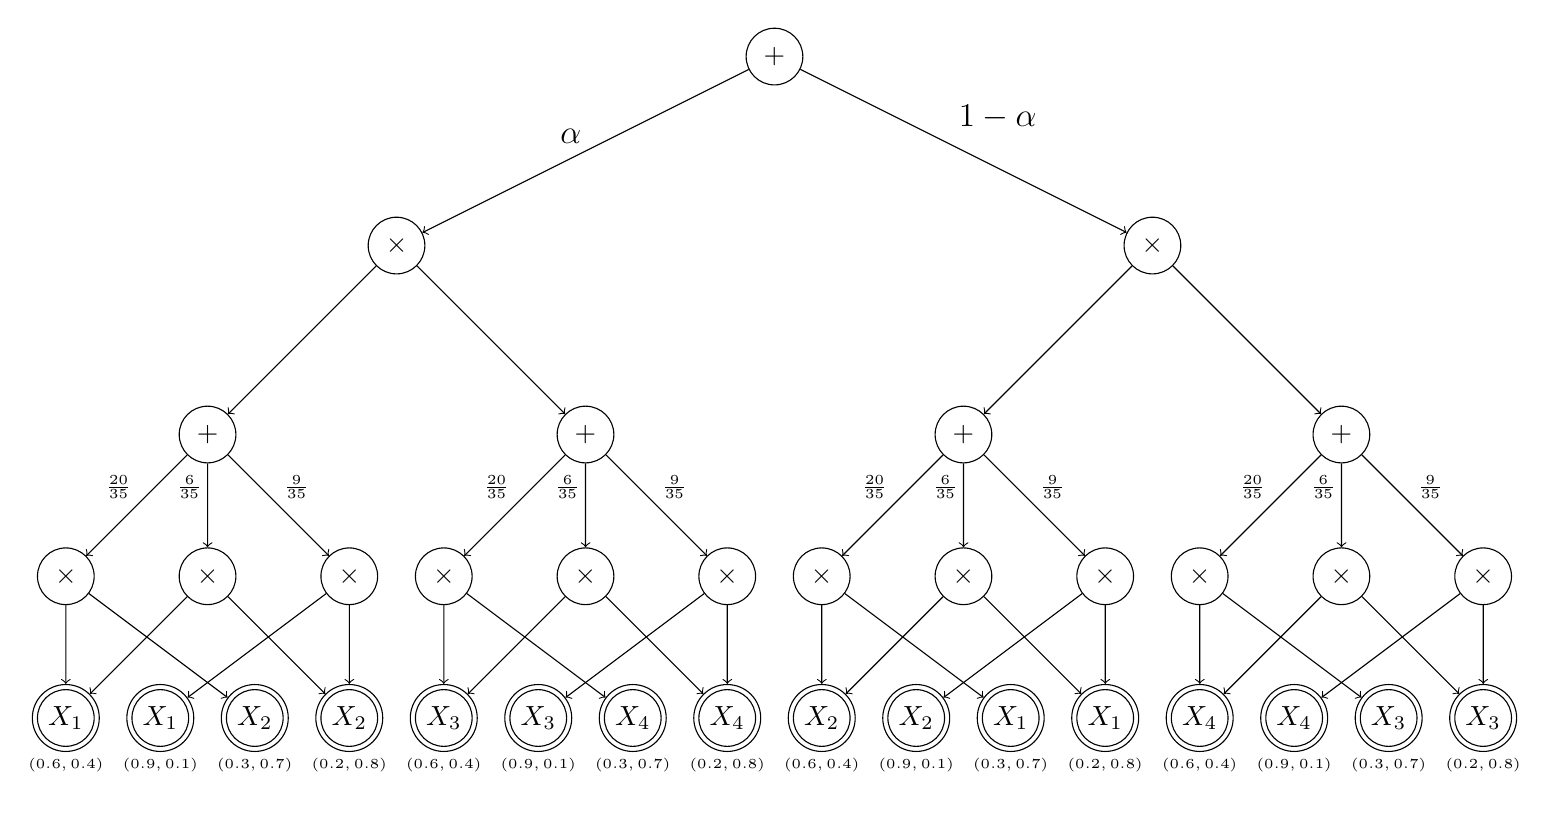
\begin{tikzpicture}
          [scale=.6,auto=left,every node/.style={draw, circle, inner sep = 0pt, minimum width = 0.72cm}]
        \node (n1) at (5,10) {$+$};
        \node (n2) at (2,7) {$\times$};
        \node (n3) at (5,7) {$\times$};
        \node (n4) at (8,7) {$\times$};
        \node (n5) at (2,4) {$X_1$};
        \node (n6) at (4,4) {$X_1$};
        \node (n7) at (6,4) {$X_2$};
        \node (n8) at (8,4) {$X_2$};

        \node[minimum width = 0.85cm] (n5) at (2,4) {};
        \node[minimum width = 0.85cm] (n6) at (4,4) {};
        \node[minimum width = 0.85cm] (n7) at (6,4) {};
        \node[minimum width = 0.85cm] (n8) at (8,4) {};

        \node[draw=none] (n9) at (2,3) {\tiny $(0.6, 0.4)$};
        \node[draw=none] (n10) at (4,3) {\tiny $(0.9, 0.1)$};
        \node[draw=none] (n11) at (6,3) {\tiny $(0.3, 0.7)$};
        \node[draw=none] (n12) at (8,3) {\tiny $(0.2, 0.8)$};

        \foreach \from/\to/\weight/\pos in {n1/n2/$\frac{20}{35}$/above left, n1/n3/$\frac{6}{35}$/above left, n1/n4/$\frac{9}{35}$/above right}
          \draw (\from) edge[->] node[\pos, draw=none, circle=none, minimum width=0.5cm, minimum height=0.2cm, inner sep=2pt]{\scriptsize \weight} (\to);

        \foreach \from/\to in {n2/n5, n2/n7, n3/n5, n3/n8, n4/n6, n4/n8}
          \draw (\from) edge[->] (\to);

        \node (m1) at (13,10) {$+$};
        \node (m2) at (10,7) {$\times$};
        \node (m3) at (13,7) {$\times$};
        \node (m4) at (16,7) {$\times$};
        \node (m5) at (10,4) {$X_3$};
        \node (m6) at (12,4) {$X_3$};
        \node (m7) at (14,4) {$X_4$};
        \node (m8) at (16,4) {$X_4$};

        \node[minimum width = 0.85cm] (m5) at (10,4) {};
        \node[minimum width = 0.85cm] (m6) at (12,4) {};
        \node[minimum width = 0.85cm] (m7) at (14,4) {};
        \node[minimum width = 0.85cm] (m8) at (16,4) {};

        \node[draw=none] (m9) at (10,3) {\tiny $(0.6, 0.4)$};
        \node[draw=none] (m10) at (12,3) {\tiny $(0.9, 0.1)$};
        \node[draw=none] (m11) at (14,3) {\tiny $(0.3, 0.7)$};
        \node[draw=none] (m12) at (16,3) {\tiny $(0.2, 0.8)$};

        \foreach \from/\to/\weight/\pos in {m1/m2/$\frac{20}{35}$/above left, m1/m3/$\frac{6}{35}$/above left, m1/m4/$\frac{9}{35}$/above right}
          \draw (\from) edge[->] node[\pos, draw=none, circle=none, minimum width=0.5cm, minimum height=0.2cm, inner sep=2pt]{\scriptsize \weight} (\to);

        \foreach \from/\to in {m2/m5, m2/m7, m3/m5, m3/m8, m4/m6, m4/m8}
          \draw (\from) edge[->] (\to);

        \node (nm) at (9,14) {$\times$};

        \draw (nm) edge[->] (n1);
        \draw (nm) edge[->] (m1);

        \node (xn1) at (21,10) {$+$};
        \node (xn2) at (18,7) {$\times$};
        \node (xn3) at (21,7) {$\times$};
        \node (xn4) at (24,7) {$\times$};
        \node (xn5) at (18,4) {$X_2$};
        \node (xn6) at (20,4) {$X_2$};
        \node (xn7) at (22,4) {$X_1$};
        \node (xn8) at (24,4) {$X_1$};

        \node[minimum width = 0.85cm] (xn5) at (18,4) {};
        \node[minimum width = 0.85cm] (xn6) at (20,4) {};
        \node[minimum width = 0.85cm] (xn7) at (22,4) {};
        \node[minimum width = 0.85cm] (xn8) at (24,4) {};

        \node[draw=none] (xn9) at (18,3) {\tiny $(0.6, 0.4)$};
        \node[draw=none] (xn10) at (20,3) {\tiny $(0.9, 0.1)$};
        \node[draw=none] (xn11) at (22,3) {\tiny $(0.3, 0.7)$};
        \node[draw=none] (xn12) at (24,3) {\tiny $(0.2, 0.8)$};

        \foreach \from/\to/\weight/\pos in {xn1/xn2/$\frac{20}{35}$/above left, xn1/xn3/$\frac{6}{35}$/above left, xn1/xn4/$\frac{9}{35}$/above right}
          \draw (\from) edge[->] node[\pos, draw=none, circle=none, minimum width=0.5cm, minimum height=0.2cm, inner sep=2pt]{\scriptsize \weight} (\to);

        \foreach \from/\to in {xn2/xn5, xn2/xn7, xn3/xn5, xn3/xn8, xn4/xn6, xn4/xn8}
          \draw (\from) edge[->] (\to);

        \node (xm1) at (29,10) {$+$};
        \node (xm2) at (26,7) {$\times$};
        \node (xm3) at (29,7) {$\times$};
        \node (xm4) at (32,7) {$\times$};
        \node (xm5) at (26,4) {$X_4$};
        \node (xm6) at (28,4) {$X_4$};
        \node (xm7) at (30,4) {$X_3$};
        \node (xm8) at (32,4) {$X_3$};

        \node[minimum width = 0.85cm] (xm5) at (26,4) {};
        \node[minimum width = 0.85cm] (xm6) at (28,4) {};
        \node[minimum width = 0.85cm] (xm7) at (30,4) {};
        \node[minimum width = 0.85cm] (xm8) at (32,4) {};

        \node[draw=none] (xm9) at (26,3) {\tiny $(0.6, 0.4)$};
        \node[draw=none] (xm10) at (28,3) {\tiny $(0.9, 0.1)$};
        \node[draw=none] (xm11) at (30,3) {\tiny $(0.3, 0.7)$};
        \node[draw=none] (xm12) at (32,3) {\tiny $(0.2, 0.8)$};

        \foreach \from/\to/\weight/\pos in {xm1/xm2/$\frac{20}{35}$/above left, xm1/xm3/$\frac{6}{35}$/above left, xm1/xm4/$\frac{9}{35}$/above right}
          \draw (\from) edge[->] node[\pos, draw=none, circle=none, minimum width=0.5cm, minimum height=0.2cm, inner sep=2pt]{\scriptsize \weight} (\to);

        \foreach \from/\to in {xm2/xm5, xm2/xm7, xm3/xm5, xm3/xm8, xm4/xm6, xm4/xm8}
          \draw (\from) edge[->] (\to);

        \node (xnm) at (25,14) {$\times$};

        \draw (xnm) edge[->] (xn1);
        \draw (xnm) edge[->] (xm1);

        \node (x) at (17,18) {$+$};

        \draw (x) edge[->] node[above left, draw=none, circle=none, minimum width=0.5cm, minimum height=0.2cm, inner sep=2pt]{\large $\alpha$} (nm);
        \draw (x) edge[->] node[above right, draw=none, circle=none, minimum width=0.5cm, minimum height=0.2cm, inner sep=2pt]{\large $1-\alpha$} (xnm);
      \end{tikzpicture}
    }

    (a)
  \end{minipage}\begin{minipage}{0.35\textwidth}
    \centering
    \scalebox{0.6}{
      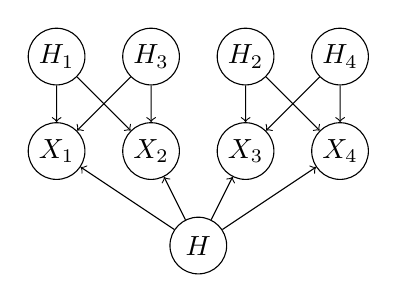
\begin{tikzpicture}
          [scale=.6,auto=left,every node/.style={draw, circle, inner sep = 0pt, minimum width = 0.72cm}]
        \node (h1) at (3,7) {$H_1$};
        \node (x1) at (3,5) {$X_1$};

        \node (h3) at (5,7) {$H_3$};
        \node (x2) at (5,5) {$X_2$};

        \node (h2) at (7,7) {$H_2$};
        \node (x3) at (7,5) {$X_3$};

        \node (h4) at (9,7) {$H_4$};
        \node (x4) at (9,5) {$X_4$};

        \foreach \from/\to in {h1/x2, h2/x3, h2/x4, h3/x2, h4/x3, h4/x4}
          \draw (\from) edge[->] (\to);

        \node (h) at (6,3) {$H$};

        \foreach \from/\to in {h/x2, h/x3, h/x4}
          \draw (\from) edge[->] (\to);

        \foreach \from/\to in {h/x1, h1/x1, h3/x1}
          \draw (\from) edge[->] (\to);
      \end{tikzpicture}
    }

    (b)
  \end{minipage}

  \caption{
    \textbf{(a)} SPN $\mathcal{U}$ construída duplicando a SPN $\mathcal{T}$ da figura \ref{fig:ex1} (a) e adicionando um nó soma que aponta para a SPN original e sua cópia.
    \textbf{(b)} Estrutura da rede bayesiana construída por meio da conversão da SPN $\mathcal{U}$ usando algoritmo de Zhao \emph{et al.}
  }
  \label{fig:ex2}
\end{figure}

\section{Conclusões}

O artigo de Zhao \emph{et al.} \cite{Zhao2015} mostra que embora a rede bayesiana resultante da conversão tenha estrutura simples (bipartida), é possível relacionar a profundidade de uma SPN com a \emph{treewidth} da rede bayesiana convertida. Isso indica que mais camadas numa rede soma-produto implicam num \emph{treewidth} maior para a rede bayesiana e portanto uma SPN com mais camadas pode representar distribuições mais complexas.

Além disso, ele esclarece que pode haver outras técnicas para converter uma SPN numa BN com uma representação mais compacta e um \emph{treewidth} menor. De fato, ele não prova que seu algoritmo é a única forma de fazê-lo.

No mais, um resultado importante desse trabalho é que a partir dele pode-se usar algoritmos para aprender estrutura e parâmetros de redes soma-produto para aprender redes bayesianas com diagramas de decisão algébrica.
